% !Mode:: "TeX:UTF-8"
\documentclass[13pt,fontset=mac]{ctexbeamer}
\usepackage[utf8]{inputenc}


\usepackage{amsmath,amssymb,amsthm}             % AMS Math
%\usepackage[T1]{fontenc}
\usepackage{graphicx}
\usepackage{epstopdf}
\usepackage{tikz}
\linespread{1.3}

\usepackage{mathrsfs}  %花写字母
 

%%%=== theme ===%%%
% \usetheme{Warsaw}
%\usetheme{Copenhagen}
%\usetheme{Singapore}
\usetheme{Madrid}
%\usefonttheme{professionalfonts}
%\usefonttheme{serif}
% \usefonttheme{structureitalicserif}
%%\useinnertheme{rounded}
%%\useinnertheme{inmargin}
\useinnertheme{circles}
%\useoutertheme{miniframes}
\setbeamertemplate{navigation symbols}{}
%\setbeamertemplate{footline}[page number]
\setbeamertemplate{footline}[frame number] 


%\usepackage[fontset=mac]{ctex}
%\usepackage{ctex}


\usepackage{hyperref}
\usepackage{tipa}

\titlegraphic{
\includegraphics[width=2cm]{tjnu.jpg}} 

\setbeamertemplate{theorems}[numbered]
\newtheorem{thm}{定理}
\newtheorem{lem}{引理}
\newtheorem{exa}{例}
\newtheorem*{theo}{定理}
\newtheorem*{conj}{猜想}
\newtheorem*{defi}{定义}
\newtheorem*{coro}{推论}
\newtheorem*{ex}{练习}
\newtheorem*{rem}{注}
\newtheorem*{prop}{性质}
\newtheorem*{qst}{问题}

\def\qed{\nopagebreak\hfill{\rule{4pt}{7pt}}\medbreak}
\def\pf{{\bf 证明~~ }}
\def\sol{{\bf 解~~ }}



\def\R{\mathbb{R}}
\def\Rn{\mathbb{R}^n}
\def\A{\mathscr{A}}
\def\B{\mathscr{B}}
\def\D{\mathscr{D}}
\def\E{\mathscr{E}}
\def\O{\mathscr{O}}

\def\rank{\operatorname{rank}}
\def\dim{\operatorname{dim}}
\def\0{\mathbf{0}}
\def\a{\alpha}
\def\b{\beta}
\def\r{\gamma}

\usepackage{color}
\definecolor{linkcol}{rgb}{0,0,0.4}
\definecolor{citecol}{rgb}{0.5,0,0}

\definecolor{blue}{rgb}{0,0.08,1}
\newcommand{\blue}{\textcolor{blue}}

  \usepackage{graphicx}
  \DeclareGraphicsExtensions{.eps}
%   \usepackage[a4paper,pagebackref,hyperindex=true,pdfnewwindow=true]{hyperref}


\begin{document}



\title[]{论文写作指导}
\author[]{{\large 张彪} }
\institute[]{{\normalsize
		天津师范大学\\[6pt]
		zhang@tjnu.edu.cn}}

\date{}


%
%\AtBeginSection[]
%{
%\begin{frame}
%	\frametitle{Outline}
%	\tableofcontents[currentsection]
%\end{frame}
%\setcounter{exa}{0}
%\setcounter{equation}{0}
%}



\begin{frame}
\maketitle
\end{frame}


\begin{frame}
	\frametitle{\textcolor{orange}{Outline}}
	\tableofcontents
\end{frame}




\section{LaTeX}


\begin{frame}
	\begin{itemize}
	\item 	TeX
($\backslash$t\textepsilon x$\backslash$,常被读作$\backslash$t\textepsilon k$\backslash$,音译“泰赫”,“泰克”,写作“TEX”)

\item 它在学术界特别是数学、物理学和计算机科学界十分流行。
	\item
TeX被普遍认为是一个优秀的排版工具,尤其是对于复杂数学公式的处理。
	\item
利用LaTeX等终端软件,TeX就能够排版出精美的文本以帮助人们辨认和查找。
\end{itemize}
\end{frame}


\begin{frame}{TeX}
	
	
	\begin{columns}[c]  %开始进入分栏环境,居中设置
		
		\column{6cm}
		
		\begin{itemize}
			\item
			TeX
			是一个由美国计算机教授高德纳(Donald Ervin Knuth)编写的排版软件。
			
			\item 高德纳最早开始自行编写TeX的原因,是因为当时的电脑排版技术十分粗糙,已经影响到他的巨著《计算机程序设计艺术》的印刷质量。他以典型的黑客思维模式,决定自行编写一个排版软件:TeX。
		\end{itemize}
		
		
		%\rightline{ {\Large 一华罗庚 \qquad \qquad\qquad}}
		\column{5cm} 
		\begin{figure}[p]
			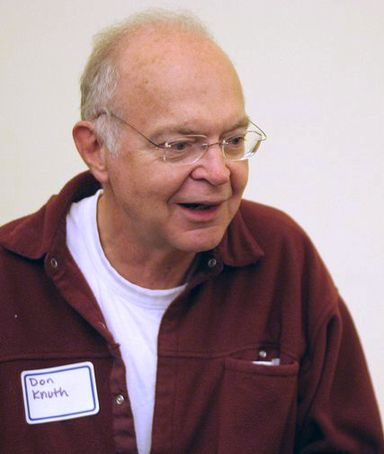
\includegraphics[scale=0.5]{Knuth.jpg}
			\caption{Donald Knuth(1938-~~)}
		\end{figure}
		
	\end{columns}
	
	
\end{frame}


\begin{frame}{LaTeX}
	\begin{columns}[c]  %开始进入分栏环境,居中设置
		
		\column{6cm}
		
\begin{itemize}
	\item LaTeX,是一种基于TEX的排版系统,由美国计算机科学家Leslie~ Lamport~(2013年获图灵奖)在20世纪80年代初期开发。
	\item 利用这种格式系统的处理,即使用户没有排版和程序设计的知识也可以充分发挥由TEX所提供的强大功能,不必一一亲自去设计或校对,能在几天,甚至几小时内生成很多具有书籍质量的印刷品。
\end{itemize}
		
	
		\column{5cm} 
		\begin{figure}[p]
			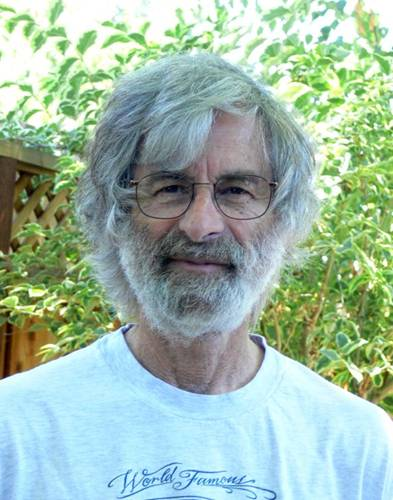
\includegraphics[scale=0.4]{Lamport.jpg}
			\caption{Lamport(1941-~~)}
		\end{figure}
		
	\end{columns}


\end{frame}

\begin{frame}{LaTeX}
\begin{itemize}
	\item 对于生成复杂表格和数学公式,这一点表现得尤为突出。因此它非常适用于生成高印刷质量的科技和数学、物理文档。这个系统同样适用于生成从简单的信件到完整书籍的所有其他种类的文档。
	\item LaTeX使用TeX作为它的格式化引擎,当前的版本是LaTeX2e(写作“LATEX2ε”)。
\end{itemize}
\end{frame}

\begin{frame}{LaTeX 发音和书写}
	\begin{itemize}
\item 	由于TEX一词应该读作“泰赫”($\backslash$t\textepsilon x$\backslash$),所以LATEX一词可以音译为“拉泰赫”。
\item 
	在英语中,IATEX实际通常读作
$\backslash$le\i t\textepsilon k$\backslash$
(音译“莱泰克”)或者(音译“拉泰克”)
$\backslash$l\textscripta\textlengthmark t\textepsilon k$\backslash$
\item 
	LATEX的开发者Lamport表示对LATEX的读音没有偏好。
		\end{itemize}
	\vspace{15pt}
		\begin{itemize}
\item 
LaTeX的正确的写法是
\begin{center}

\includegraphics[scale=0.08]{LATEX.jpg}
\end{center}
如果因技术限制而无法做到,则应该写成“LaTeX”。
\item 
不得改变任何一个字母的大小写,以免和“latex” (乳胶) 混淆。
	\end{itemize}

	
	

	
	

\end{frame}



\begin{frame}{CTeX 套装}


\begin{itemize}
	\item 网站  http://www.ctex.org/
%	\item CTeX 套装是科学院吴凌云研究员的个人作品。
	\item 在 CTeX 套装刚刚问世之时,因其解决了繁琐的中文字体安装工作,所以广受欢迎。
\end{itemize}
 但是,
\begin{itemize}
	\item  一方面 CTeX 套装已经很久不更新(最新的稳定版本	v2.9.2.164 -- 2012.03.22),内里的宏包、工具陈旧;
	\item 另一方面,随着 XeLaTeX 的发展,以及 xeCJK 等技术的成熟,上述这些繁琐的工作已经没有必要而失去意义;
\end{itemize}

	因此,\alert{现在不推荐使用 CTeX 套装}。
	


%不要安装和使用 CTeX 套装!
%如\documentclass{ctexart}
\end{frame}



\begin{frame}
{CTeX 宏集}
\begin{itemize}
	\item 
虽然它的名字也是「CTeX」,但是 CTeX 宏集和 CTeX 套装是两个不同的东西。
\item  CTEX 宏集支持LATEX、pdfLATEX、XƎLATEX、LuaLATEX、upLATEX 等多种不同的编译方式,并为它们提供了统一的界面。主要功能由宏包ctex 以及中文文档类ctexart、ctexrep、ctexbook 和 ctexbeamer 实现。
\item 我们推荐\alert{优先使用 CTeX 宏集处理中文}。
\item 中文的文档可以直接使用ctex 文档类。
%也就是ctexart、ctexrep、ctexbook、ctexbeamer 这些。
\end{itemize}

 
%请在任何情况下优先使用 CTeX 宏集在 LaTeX 中处理中文!
\end{frame}


\begin{frame}{推荐使用TeXLive + TeXStudio }
	推荐安装最新版本的
	
	\begin{itemize}
		\item TeXLive 
		
		\href{https://www.tug.org/texlive/}{https://www.tug.org/texlive/}
		
		
		
		\item TeXStudio
		
		http://www.texstudio.org/
	\end{itemize}
	
	TeXLive + TeXStudio  ~安装指南,可以参考
	\begin{itemize}
		\item 	\href{https://zhuanlan.zhihu.com/p/80603542}{https://zhuanlan.zhihu.com/p/80603542}
		\item \href{https://blog.csdn.net/yeler082/article/details/80665186}{https://blog.csdn.net/yeler082/article/details/80665186}
	\end{itemize}
\end{frame}




\begin{frame}
{ 编译器: TeX Live}

\begin{itemize}
	\item TeX Live 是 TUG (TeX User Group) 维护和发布的 TeX 系统,可说是「官方」的 TeX 系统。
	\item 我们推荐任何阶段的 TeX 用户,都尽可能使用 TeX Live,以保持在跨操作系统平台、跨用户的一致性。
	\item TeX Live 的官方站点是 \href{https://tug.org/texlive/}{https://tug.org/texlive/}
	\item 建议尝试使用国内大学的镜像站下载。
	
	\href{https://mirrors.ustc.edu.cn/CTAN/systems/texlive/Images/} {https://mirrors.ustc.edu.cn/CTAN/systems/texlive/Images/}
	
	
	\href{https://mirrors.tuna.tsinghua.edu.cn/CTAN/systems/texlive/Images/}{https://mirrors.tuna.tsinghua.edu.cn/CTAN/systems/texlive/Images/}
	
\end{itemize}
\end{frame} 

\begin{frame}{编辑器}
\begin{itemize}
\item  TeXStudio (推荐使用)
\item TeXmaker
\item TeXworks (TexLive自带)
\item TexPad (for Mac users)
\end{itemize}
\end{frame}



\section{Mathpix}
\begin{frame}{Mathpix}
\begin{itemize}
	\item  Mathpix
	
\href{https://mathpix.com/}{https://mathpix.com/}
\end{itemize}
\end{frame} 


\section{JabRef}
\begin{frame}{JabRef}
\begin{itemize}
\item  Jabref

\href{https://www.jabref.org/}{https://www.jabref.org/}
\end{itemize}
\end{frame} 
\end{document} 